% Chapter 1

\chapter{Project 1: Binary Search} % Main chapter title

\label{Chapter1} % For referencing the chapter elsewhere, use \ref{Chapter1} 

\lhead{Chapter 1. \emph{Binary Search}} % This is for the header on each page - perhaps a shortened title

%----------------------------------------------------------------------------------------

\section{Introduction}



\section{Implementations}
The following four implementations of the binary search algorithm used four different memory layouts. The tree structures are shown in figure \ref{fig:memory_layouts}.

\begin{figure}[htbp]
	\centering
		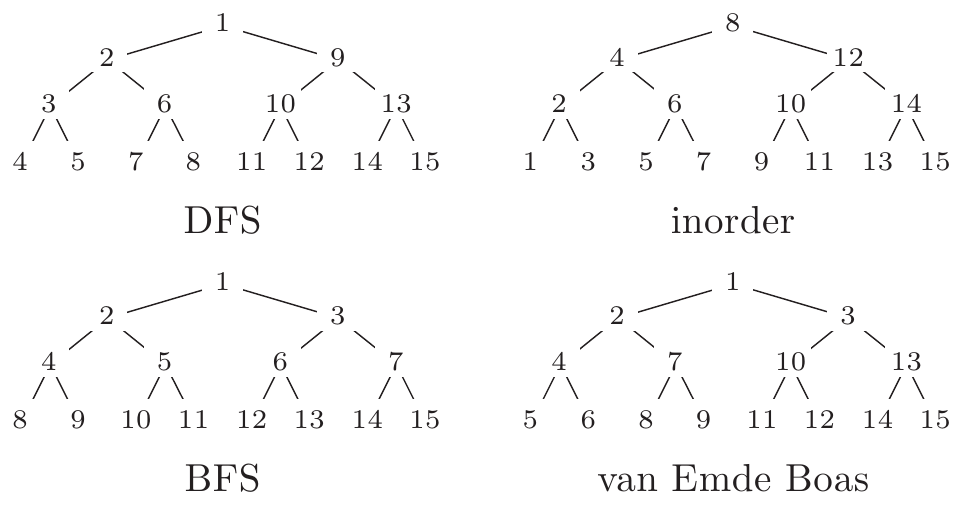
\includegraphics[width=\textwidth]{./Figures/Project1/MemoryLayouts.png}
		\rule{35em}{0.5pt}
	\caption[Memory layouts]{
	The four different tree structures shows the memory layout used in the implementations. The figure is taken from \citep{binAlg}.
	}
	\label{fig:memory_layouts}
\end{figure}


\subsection{Linear search}
To compare the running times for the algorithms, we have implemented a linear search function.
\begin{verbatim}
For each item in the list:
     if that item has the desired value,
         stop the search and return the item's location.
\end{verbatim}
 Return -1\footnote{We return -1 if the element dosn't exist in the list}.
 \begin{lstlisting}[numbers=left]
 // Check result
if (oldRes != -1 && oldRes != newRes) {
	printf("Wrong result. prev:%s %d, new:%s %d, ArrSize %d, searchFor %d\n", algo_labels[iAlg-1], oldRes, algo_labels[iAlg], newRes, arrSize, searchFor); 
 					
}
oldRes = newRes;
\end{lstlisting}
We compare the results for the different algorithms in our test

\subsection{Inorder}

We have made a inorder binary search to compare with BFS, DFS and vEB.
Inorder is made iterative.
\lstinputlisting[language=C++, firstline=32, lastline=51, numbers=left]{./Figures/BinarySearch.cpp}
We begin by defining low, high and smallestSoFar.

In line 8 we make a while-loop, we run while high is greater than low.

We start by looking at the element whom is in the middle of the array.
If that element is smaller than the one we are looking for we set low to point at the middle +1.
If we are in the opposite case we set high to point at the middle -1.

The idea is that the array all the time is divided into one half the size where low will point at the first element in the new array and high will point at the last.

We continue until we find the element we are looking for or we return -1 if our list dosn't contain it.

\subsection{Breadth-first search (BFS)}


The following is a recursive method for filling out the bfs tree. The method is called by ``insert(0)''.
\begin{verbatim}
void insert(int bfsIndex){
  if (bfsIndex >= SIZE) return;
  insert(2*bfsIndex+1); // Left child
  bfsArray[bfsIndex] = *(linArray+linIndex);
  linIndex++;
  insert(2*bfsIndex+2); // Right child
}
\end{verbatim}


The binary search is then implemented as follows:
\begin{verbatim}
  int i = 0;
  int curr = bfsArray[i];  // The current node visited
  int res = -1;  // The latest element smaller than 'elem'.
  while (curr != elem){
    i = 2*i+1;  // Left child
    if (curr < elem){
      i++;  // Right child (=left+1)
      res = curr;  // This is now the latest known element smaller than 'elem'.
    }
    // If we have reached a bottom node, return the last element lower than 'elem'.
    if (i >= SIZE){
      return res;
    }
    curr = bfsArray[i];
  }
  // At this point, the while loop did not continue because curr==elem
  return curr;
\end{verbatim}




\subsection{Depth-first search (DFS)}


\subsection{Van Emde Boas (vEB)}

The vEB array is constructed using the following recursive method. It is called using ``insert(0,0,0,roots)'' where roots is an array of the same size as the depth of the tree.

\begin{verbatim}
void insert(int vebIndex, int atDepth, int depthIndex, int roots[]){
  if (vebIndex >= size || vebIndex < 0) {
    return;
  }
  int rootIndex = findPosition((~atDepth+1) & atDepth); // findRightmostOne(atDepth)
  int depthType = findPosition(~atDepth & (atDepth+1)); // findRightmostZero(atDepth)
    
  int rootsNew[depth];
  for (int i=0; i<depth; i++){
      if (i <= rootIndex) rootsNew[i] = vebIndex;
      else rootsNew[i] = roots[i];
  }

  int amount = 1<<((1<<depthType)-1);
  int vebLeft = (2*(depthIndex & (amount-1)) +1) * (2*amount -1) + rootsNew[depthType];

  insert(vebLeft, atDepth+1, 2*depthIndex, rootsNew); // Left child
    
  vebArray[vebIndex] = *(linArray+linIndex);
  linIndex++;

  int vebRight = vebLeft + 2*amount -1;
  insert(vebRight, atDepth+1, 2*depthIndex+1, rootsNew); // Right child
}
\end{verbatim}


The binary search is implemented as follows:
\begin{verbatim}
  int vebIndex = 0;
  int curr = vebArray[vebIndex]; // The current node visited
  int res = -1; // The latest element smaller than 'elem'.
  int atDepth = 0;
  int depthIndex = 0;
  int roots[depth];
  for (int i=0; i<depth; i++){
      roots[i] = 0;
  }
    
  while (curr != elem){
    int rootIndex = findPosition((~atDepth+1) & atDepth); // findRightmostOne(atDepth)
    int depthType = findPosition(~atDepth & (atDepth+1)); // findRightmostZero(atDepth)

    for (int i=0; i<=rootIndex; i++){
	roots[i] = vebIndex;
    }
    int goRight = curr < elem;
    int amount = 1<<((1<<depthType)-1);
    vebIndex = (2*(depthIndex & (amount-1)) +1 + goRight) * (2*amount -1) + roots[depthType];

    if (goRight){
      res = curr;  // This is now the latest known element smaller than 'elem'.
    }
    if (vebIndex >= size || vebIndex < 0){
      return res;
    }
    atDepth++;
    depthIndex = 2*depthIndex + goRight;
    curr = vebArray[vebIndex];
  }
  // At this point, the while loop did not continue because curr==elem
  return curr;
\end{verbatim}








\section{Results and discussion}



\begin{figure}[htbp]
	\centering
		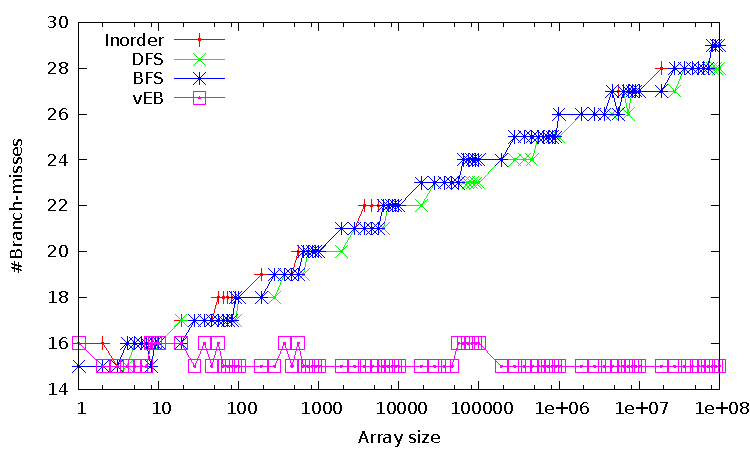
\includegraphics[width=\textwidth]{./Figures/Project1/Branch_misses.pdf}
		\rule{35em}{0.5pt}
	\caption[Branch misses]{
	Bla bla bla.
	}
	\label{fig:Branch_misses}
\end{figure}


\begin{figure}[htbp]
	\centering
		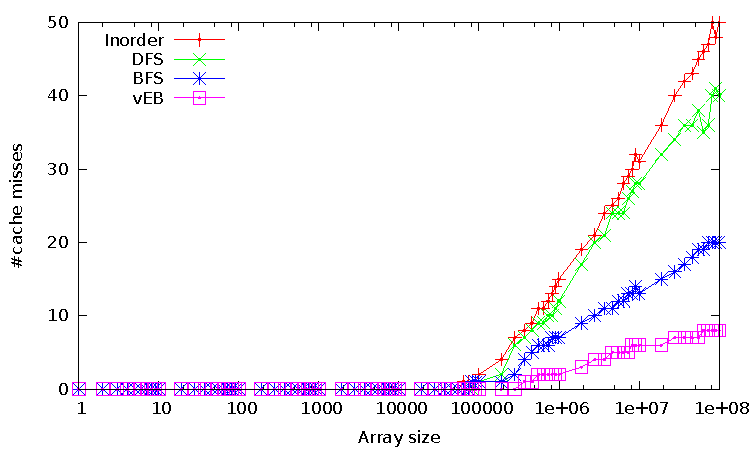
\includegraphics[width=\textwidth]{./Figures/Project1/Cache_misses.pdf}
		\rule{35em}{0.5pt}
	\caption[Cache misses]{
	Bla bla bla.
	}
	\label{fig:Cache_misses}
\end{figure}



\begin{figure}[htbp]
	\centering
		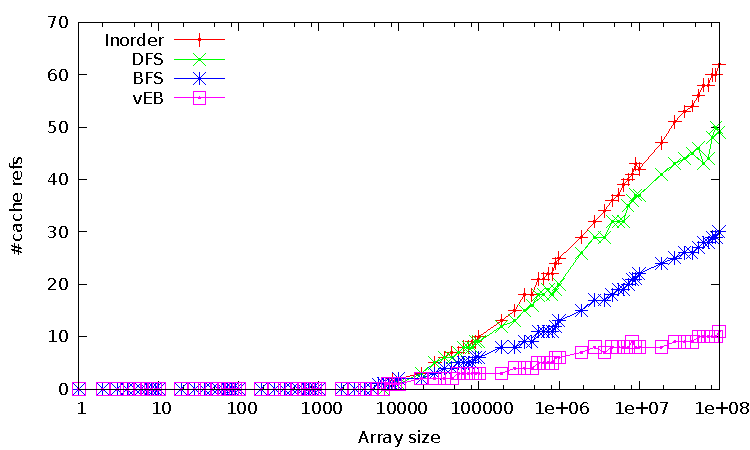
\includegraphics[width=\textwidth]{./Figures/Project1/Cache_refs.pdf}
		\rule{35em}{0.5pt}
	\caption[Cache refs]{
	Bla bla bla.
	}
	\label{fig:Cache_refs}
\end{figure}



\begin{figure}[htbp]
	\centering
		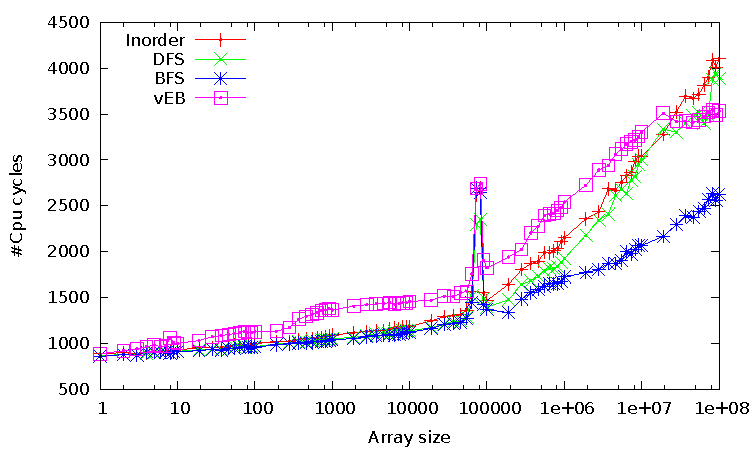
\includegraphics[width=\textwidth]{./Figures/Project1/Cpu_cycles.pdf}
		\rule{35em}{0.5pt}
	\caption[CPU cycles]{
	Bla bla bla.
	}
	\label{fig:Cpu_cycles}
\end{figure}


\begin{figure}[htbp]
	\centering
		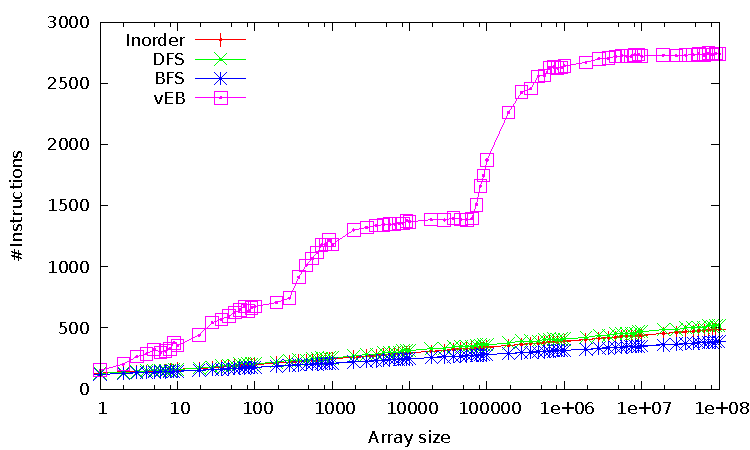
\includegraphics[width=\textwidth]{./Figures/Project1/Instructions.pdf}
		\rule{35em}{0.5pt}
	\caption[Instructions]{
	Bla bla bla.
	}
	\label{fig:Instructions}
\end{figure}

